\chapter{Problemforståelse}
Denne fasen eksisterer for å passe på at en har forstått problemet i dypere detalj. Verktøyene som er relevante å bruke skal gi en bedre forståelse av blant annet omfanget og de ulike aspektene ved et problem. Jo bedre tilgang en har på informasjon, logger og dokumentasjon, jo bedre vil denne fasen kunne utføres. 


\section{Ytelsesmatrise}
Ytelsesmatrise er et diagram som tar i betraktning den nåværende ytelsen til en variabel. Dette kan bety flere ting og vurderes i ulike former, men i dette caset definerer vi ytelse som hvor godt de ulike variablene fungerer i dag. Det som gjør ytelsesmatrise så nyttig er at den også vurderer viktigheten, slik at en kan vurdere hvilken prioritering variablene som blir analysert har. I dette caset blir viktighet definert som hvor funksjonskritisk ressursene er for arbeidet som gjøres ved NTNU.

\subsection{Ønsket utbytte}
Ved bruk av dette verktøyet er det ønskelig å undersøke hvordan eksisterende kontroller fungerer i forhold til deres viktighet for NTNU. 

\subsection{Gjennomføring}
Prosessen startet ved å finne ut hvilke aspekter av problemet som skulle vurderes. Gruppen kom fram til å vurdere formene for kontroller som stopper eller reduserer sjansen for at trusselaktørene misbruker NTNU sin infrastruktur. 

Disse skulle vurderes basert på viktighet og ytelse. 

Matrisen ble tegnet opp i Excel der hver akse ble konstruert fra en til ni, og matrisen ble delt inn i fire områder:
\begin{description}
    \item[Uviktig:] Når både viktigheten og ytelsen er fra en til fem.
    \item[Overdrevent:] Når viktigheten er fra en til fem og ytelsen er fra fem til ni.
    \item[Ok:] Når både viktigheten og ytelsen er fra fem til ni.
    \item[Må forbedres:] Når viktigheten er fra fem til ni, mens ytelsen bare er fra en til fem.
\end{description}

\subsection{Resultater}
Variablene som ble vurdert til å kunne hjelpe til å redusere utvinning av kryptovaluta hos NTNU er som følger:
\begin{description}
    \item[Adgangskontroll på HPC klynger:] Klynger av tilkoblet maskinvare som sammen utgir svært høy ytelse. Er også kjent som superdatamaskiner. Disse er godt beskyttet med streng adgangskontroll og logging av alt som blir gjort.
    \item[Adgangskontroll på kritiske servere:] Adgangskontroll til servere som har en funksjonskritisk og/eller virksomhetskritisk rolle i driften av NTNU, som for eksempel DNS og DHCP servere. 
    \item[Adgangskontroll på andre servere:] Adgangskontroll til alle servere som ikke har en kritisk rolle i NTNU, men som fortsatt kan bli misbrukt. Inkluderer servere som står åpent ut mot nettet. 
    \item[Beskyttelse mot ufrivillig utvinning på datamaskiner:] Personer får tilgang til din datamaskin gjennom nettleseren og bruker den til å utvinne kryptovaluta. 
    \item[Policy på hva som er akseptabelt som BYOD:] Definerer hva som er lov å ta med av BYOD.
    \item[IT-reglement på krypto utvinning:] IT-reglementet spesifiserer per idag bare at det å bruke universitetets ressurser til kommersiell virksomhet ikke er greit. Det kan være vanskelig for folk å ta koblingen til at strøm er en slik ressurs og at utvinning av kryptovaluta kan regnes som kommersiell virksomhet. Sånn som IT-reglementet er idag er det heller ikke noen gode sanksjonsmuligheter mot folk som utvinner kryptovaluta.

\end{description}

Under ser vi hvor de ulike ressursene, eller aktiva, er plassert i henhold til de tidligere nevnte områdene.
\begin{figure}[H]
    \centering
    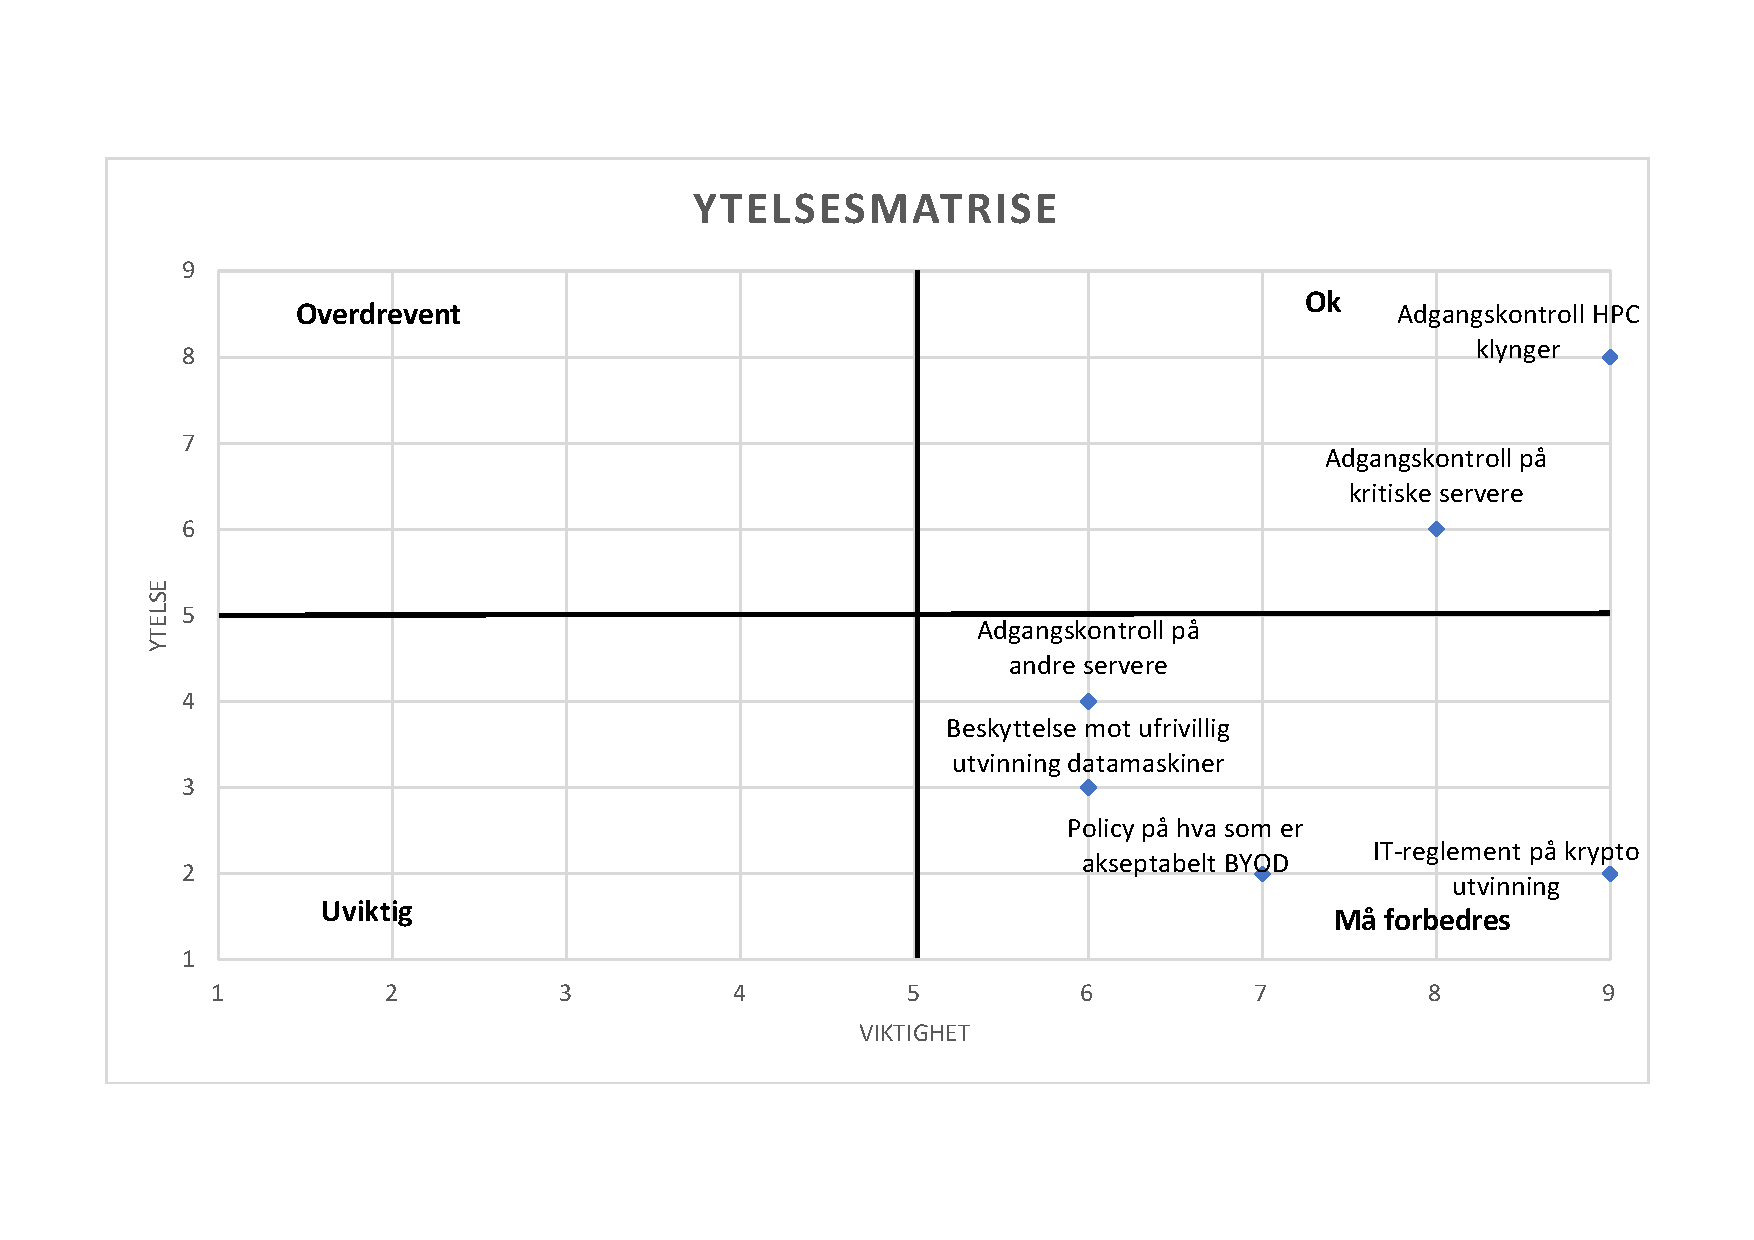
\includegraphics[scale=0.5]{case_3/bilder/ytelsesmatrise.pdf}
    \caption[Ytelsesmatrise]{Resultater fra ytelsesmatrisen}
    \label{fig:ytelsesmatrise}
\end{figure}

Det er mest kritisk å vurdere de variablene som havner under ``må forbedres''. Selv om noen havner under ``ok'', bør de fortsatt vurderes, men de vil ha lavere prioritet enn de nevnt over. Variabler som er uviktig eller overdrevent trenger man ikke vurdere nøye. Matrisen viser følgende prioriteringsgrunnlag til utbedring:

\begin{enumerate}
    \item IT-reglement på krypto utvinning
    \item Policy på hva som er greit som BYOD (IT-regement på BYOD som driver med utvinning)
    \item Beskyttelse mot ufrivillig utvinning på datamaskiner
    \item Adgangskontroll på andre servere
    \item Adgangskontroll på kritiske servere
    \item Adgangskontroll på HPC klynger
\end{enumerate}

\subsection{Konklusjon av verktøyet}
Verktøyet var nyttig for å finne frem til et prioritetsgrunnlag for de ulike enhetene som kan misbrukes eller misbruke NTNU sine ressurser. Vi ser at det er IT-reglementets mangel på spesifisering av kryptoutvinning som er det største problemet. 